\section{Practical Security}

The theoretical guarantees in the previous sections — metadata security without needing to trust
the server or the network — all assume that your local computer is completely trusted. This is unavoidable: no fancy encryption schemes will help you if your computer comes with a preinstalled backdoor. Nevertheless, while \textbf{we fundamentally cannot eliminate the client-side risk, we can reduce it}. We care about practical security as much as we care about the theoretical security. In this section, we outline the mitigations we undertake: reducing the attack surface by modularizing and supply chain protection, minimizing bugs by being open source, securing code distribution and updates, and protecting against non-privileged local malware.

We emphasize that we cannot achieve perfect security without your effort. \textbf{PLEASE DO NOT USE ANYSPHERE FOR SECURITY-CRITICAL USE CASES ON A COMPUTER YOU DO NOT TRUST}. This is especially true while we are in beta, and may have bugs.

% The Anysphere client is only as strong and secure as the most vulnerable part of our software supply chain. Software supply chains are an increasingly complex (and brittle) part of the software ecosystem because of a large and growing number of direct and transitive dependencies written across the world. 
% The Anysphere client is designed to handle extreme private and critical communication securely, so our team has enforced a high bar of security for the core of our system. We focused on providing practical protection by significantly reducing the attack surface of our client, ensuring safe updates, and protecting against non-privileged software. 

% A note on the client's security, in the context of our threat model: Anysphere trusts its client's devices. 
% In particular, we trust that the local device is running a correct implementation of our protocol, and the computer comes without pre-installed backdoors. 
% Our model is the bare minimum of trust we must assume, and we think this is reasonable given the intense focus of Apple and many other companies on device security. 
% (Put another way, no encryption schemes we can come up with can secure our client inside a compromised computer.)
% And with this context, we will present our measures to reduce the risk of a compromised Anysphere client.


\subsection{Reducing the attack surface: modularity and supply chain risk}

As illustrated in \cref{fig:systemdiagram}, our client consists of two parts: a UI frontend and a daemon backend. The daemon backend contains all security-critical code. We sandbox the UI frontend so that it is not allowed to talk to the internet. Instead, all message sending goes through the daemon. That way, bugs and malicious code on the front-end cannot compromise security.
\begin{figure*}
    \centering
    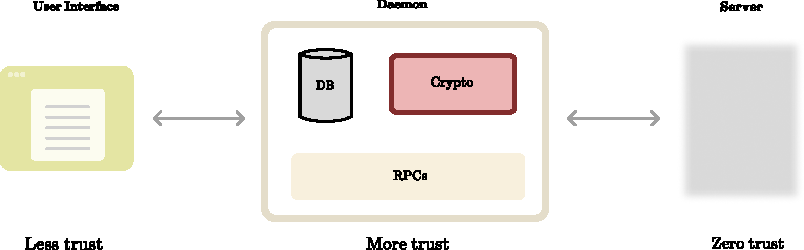
\includegraphics[width=0.8\textwidth]{systemdiagram.pdf}
\caption{System architecture. The UI and the daemon run on your local computer and require some trust assumptions. The UI is cut off from the internet, and can only communicate via the daemon, meaning that it needs lower trust assumptions. The crypto module in the daemon requires the highest level of trust, and uses the widely trusted Libsodium library.}
\label{fig:systemdiagram}
\end{figure*}
We also reduce the attack surface of the daemon itself. In particular, we take care in ensuring our dependency chain is small to protect against supply chain attacks. Many popular languages, including Rust, Go and Python, have great package managers, which led to an ecosystem where packages generally have hundred of transitively dependencies. For this reason, we chose to use \Cpp for all essential daemon code, depending only on a few well-known packages with long-term support and good security practices (Abseil, gRPC, SQLite, Libsodium). We wrote a Rust API for database interactions, being extremely careful with our dependency chain. 

\subsection{Eliminating bugs: open source}

All code that is required for security is open source. The repositories \\ {\tt \href{https://github.com/anysphere/client}{github.com/anysphere/client}} and  {\tt \href{https://github.com/anysphere/asphr}{github.com/anysphere/asphr}} contain all code for our Daemon and UI. Our server is not open source, \textit{which is justified as our threat model guarantees security no matter what code is run on our server}. 

\subsection{Code distribution and updates}

We need to ensure that our code is the code that is running on your computer. For this reason, Anysphere is not a web app — serving code on the web leads to huge vulnerabilities, and should, in our opinion, never be done for security-critical codes. The reason is that everytime you visit a website, you give attackers an opportunity to serve you malicious code. Instead, Anysphere is a local app: you download it once, and can ensure the correct code is downloaded yourself by checking the signature and hash.

%you download the cryptographic code every single time, meaning that every single time you use the website

Local apps need to be updated. Currently, we use Electron's auto-updater to perform the signature checks for us. We are actively working on building our own update verification process. In that process, two people from our team need to sign each update separately, and both signatures need to be present for your local app to accept the update. If either of us loses our key, we would not be able to push an update by design.

\subsection{Protection against non-privileged local malware}

If you've granted administrator access to a malicious program on your computer, there is, unfortunately, nothing to be done. We can, nevertheless, reduce the risk of non-privileged malware. Our beta version protects against non-privileged malware\xxx[stzh1555]{How do we achieve this?}, but in the future, we are planning to encrypt the local database, require a password to unlock the app, and use OS-level access controls to make sure only certain processes can access the daemon.

%Again, we do not aim to eliminate the risk here. Once an attacker has access to your computer, it is very, very hard to shield yourself from them.